\documentclass[12pt]{article}

\usepackage[utf8]{inputenc}
\usepackage[T1]{fontenc}
\usepackage[a4paper, margin=1in]{geometry}  
\usepackage{graphicx}
\usepackage{hyperref}
\usepackage{float} % For [H] option in figures

\title{Anotacja korpusów oraz osadzenia słów i tekstów\\Część II: Modele przestrzeni wektorowych}
\author{Autorzy: Oliwer Krupa, Adam Bednarski, Jan Masłowski, Łukasz Lenkiewicz}
\date{\today}

\begin{document}

\maketitle
\newpage

\tableofcontents
\newpage

\section{Word Embeddings}

\subsection{Osadzenia słów w anotowanym korpusie (Word2Vec i Fasttext)}

W celu zbadania i wizualizacji osadzeń słów w anotowanym korpusie, zastosowaliśmy dwie metody: \textbf{Word2Vec} oraz \textbf{FastText}. Dla obu modeli osadziliśmy słowa, a następnie zwizualizowaliśmy wyniki za pomocą algorytmu t-SNE, który redukuje wymiary danych, co pozwala na łatwiejszą analizę i porównanie rezultatów.

\subsubsection{Word2Vec}
Model \textbf{Word2Vec} został przetrenowany na korpusie tekstów polskich, a następnie osadziliśmy słowa z anotowanego korpusu, aby sprawdzić, jak różne słowa są reprezentowane w przestrzeni wektorowej. Wyniki zostały przedstawione na poniższym wykresie, gdzie kolory reprezentują różne kategorie sentymentu — niektóre słowa zostały oznaczone jako "Brak etykiety", a inne jako "Wzmacnianie".

\begin{figure}[H]
    \centering
    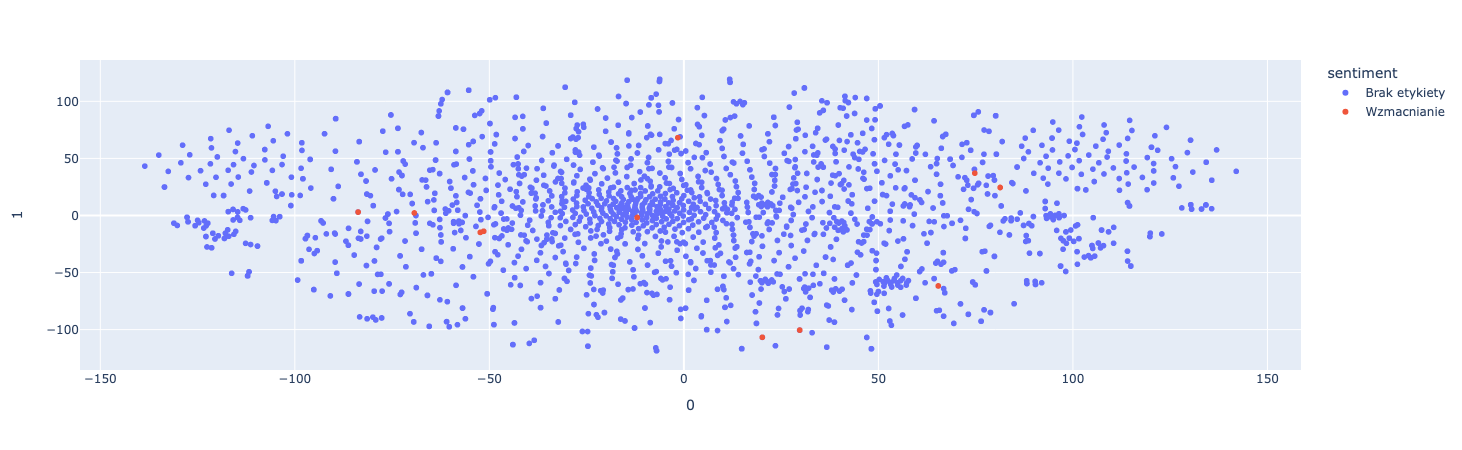
\includegraphics[width=\textwidth]{../../plots/w2v-word.png}
    \caption{Wizualizacja osadzeń słów za pomocą Word2Vec}
    \label{fig:w2v_word}
\end{figure}

Jak widać na rysunku \ref{fig:w2v_word}, większość słów jest zgrupowana w centralnej części wykresu, jednak niektóre słowa przypisane do kategorii "Wzmacnianie" znajdują się różnych obrszarach przestrzeni wektorowej.

\subsubsection{FastText}
Podobną analizę przeprowadzono z użyciem modelu \textbf{FastText}, który również został przetrenowany na korpusie polskim. Wyniki osadzeń słów z tego modelu zostały przedstawione na poniższym wykresie, który podobnie jak poprzedni, został wygenerowany za pomocą t-SNE.

\begin{figure}[H]
    \centering
    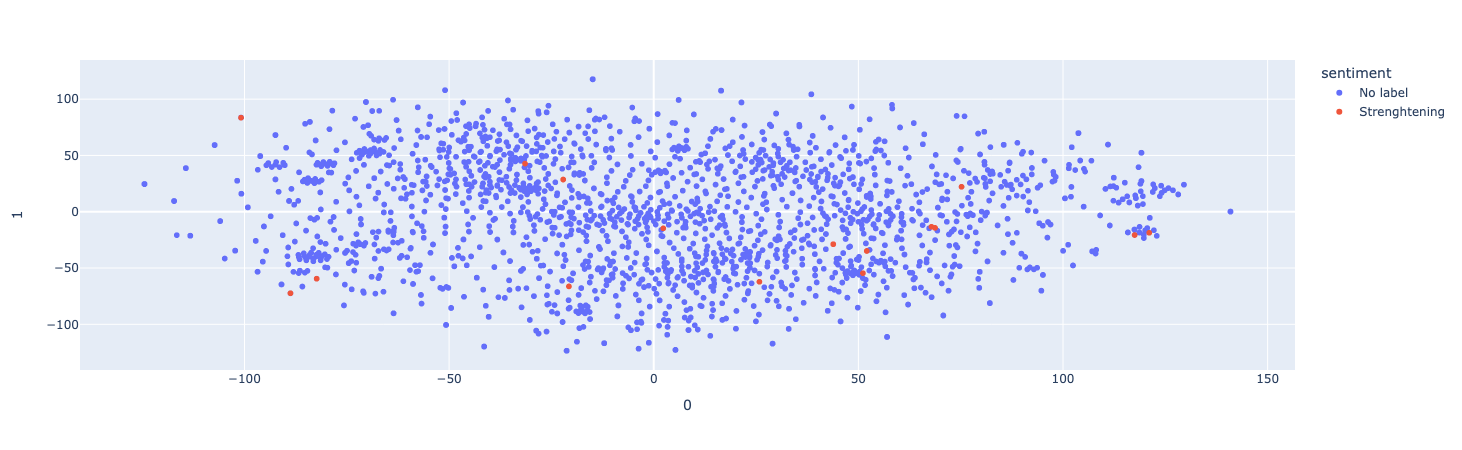
\includegraphics[width=\textwidth]{../../plots/ft-word.png}
    \caption{Wizualizacja osadzeń słów za pomocą FastText}
    \label{fig:ft_word}
\end{figure}

Rysunek \ref{fig:ft_word} pokazuje, że wyniki dla modelu FastText są podobne do tych uzyskanych z Word2Vec, chociaż niektóre grupy słów znajdują się w różnych częściach przestrzeni, co wynika z różnic w sposobie reprezentacji słów przez te dwa modele.

\subsection{Porównanie k-najbardziej podobnych słów dla modeli Word2Vec i FastText}

W ramach analizy wygenerowano listy pięciu najbardziej podobnych słów dla zaanotowanych terminów, wykorzystując modele \textbf{Word2Vec} oraz \textbf{FastText}. Wyniki pokazują różnice w sposobie modelowania podobieństw między słowami.

\subsubsection{Wyniki dla Word2Vec}
Dla modelu \textbf{Word2Vec}, lista najbardziej podobnych słów zawierała m.in.:
\begin{itemize}
    \item \textbf{by}: aby (0.89), żeby (0.86), więc (0.69)
    \item \textbf{kto}: dlaczego (0.66), czemu (0.63), jeśli (0.59)
    \item \textbf{człowiek}: osobnik (0.64), osoba (0.64), tubylec (0.62)
    \item \textbf{seks}: sexu (0.76), masturbacja (0.71), erotyka (0.63)
    \item \textbf{fakt}: stwierdzenie (0.66), twierdzenie (0.65), hipoteza (0.59)
\end{itemize}

\subsubsection{Wyniki dla FastText}
Dla modelu \textbf{FastText}, podobne słowa to:
\begin{itemize}
    \item \textbf{by}: By (0.77), żeby (0.61), muc (0.60)
    \item \textbf{kto}: Kto (0.80), ktoś (0.78), ktokolwiek (0.72)
    \item \textbf{człowiek}: Człowiek (0.80), czlowiek (0.76), człowiek. (0.69)
    \item \textbf{seks}: sex (0.80), seks. (0.78), seks- (0.76)
    \item \textbf{fakt}: faktem (0.68), faktu (0.66), Fakt (0.65)
\end{itemize}

\subsubsection{Dyskusja wyników}
Oba modele pokazują różnice w sposobie reprezentacji podobieństw. \textbf{FastText} lepiej radzi sobie z różnymi formami morfologicznymi i fleksyjnymi, np. dla słowa „człowiek” uwzględnia różne jego odmiany. Z kolei \textbf{Word2Vec} ma tendencję do generowania bardziej ogólnych podobieństw, co sprawia, że jest mniej precyzyjny w przypadku rzadkich wyrażeń. FastText dzięki n-gramom lepiej odwzorowuje złożoność morfologiczną języka polskiego.

\section{Text Embeddings}


\end{document}
